\chapter{O dinheiro forte}
\label{les:14}

\begin{chapquote}{Lewis Carroll, \textit{Alice no País das Maravilhas}}
\enquote{A primeira coisa que eu tenho que fazer}, disse Alice para si mesma, enquanto vagueava pela floresta, \enquote{é crescer até meu tamanho normal outra vez, e a segunda coisa é encontrar o caminho para aquele jardim adorável. Acho que este é o melhor plano.}
\end{chapquote}

A lição mais importante que aprendi com o Bitcoin é que, no longo prazo, o dinheiro forte é superior ao dinheiro fraco. O Dinheiro forte, também conhecido como \textit{moeda sólida}, é qualquer moeda negociada globalmente que serve como uma reserva confiável de valor.

É verdade que o Bitcoin ainda é jovem e volátil. Os críticos dirão que ele não armazena valor de forma confiável. O argumento da volatilidade está se perdendo com o tempo. A volatilidade é esperada. O mercado vai demorar um pouco para descobrir o preço justo desse novo dinheiro. Além disso, como muitas vezes é dito em tom de brincadeira, ele se baseia em um erro de medição. Se você pensar em dólares, não conseguirá ver que um bitcoin sempre será um bitcoin.

\begin{quotation}\begin{samepage}
\enquote{Uma oferta de moeda fixa, ou uma oferta alterada apenas de acordo com
critérios objetivos e calculáveis, é uma condição necessária para um preço justo significativo do dinheiro.}
\begin{flushright} -- Fr. Bernard W. Dempsey, S.J.\footnote{Perry J. Roets, S.J., \textit{Revisão da Economia Social} \cite{review-social-economy}}
\end{flushright}\end{samepage}\end{quotation}

\newpage

Como mostrou um rápido passeio pelo cemitério de moedas esquecidas, o dinheiro que pode ser impresso será impresso. Até agora, nenhum ser humano na história foi capaz de resistir a essa tentação.

O Bitcoin acaba com a tentação de imprimir dinheiro de uma forma engenhosa. O Satoshi estava ciente de nossa ganância e falibilidade --- é por isso que ele escolheu algo mais confiável do que a vontade humana: a matemática.

\begin{figure}
  \centering
  \begin{equation}
  \sum\limits_{i=0}^{32} \frac{21000 \lfloor \frac{50*10^8}{2^i} \rfloor}{10^8}
  \end{equation}
  \caption{Fórmula de suprimento do Bitcoin}
  \label{fig:supply-formula-white}
\end{figure}

Embora essa fórmula seja útil para descrever o suprimento de Bitcoin, ela não está, na verdade, em nenhum lugar do código. A emissão de novos bitcoins é feita de forma controlada por algoritmos, reduzindo a recompensa que é paga aos mineradores a cada quatro anos~\cite {btcwiki:supply}. A fórmula acima é usada para resumir rapidamente o que está acontecendo por de trás, nos bastidores. O que realmente acontece pode ser visto com mais facilidade observando a mudança na recompensa do bloco, a recompensa paga a quem encontrar um bloco válido, que acontece aproximadamente a cada 10 minutos.

\begin{figure}
  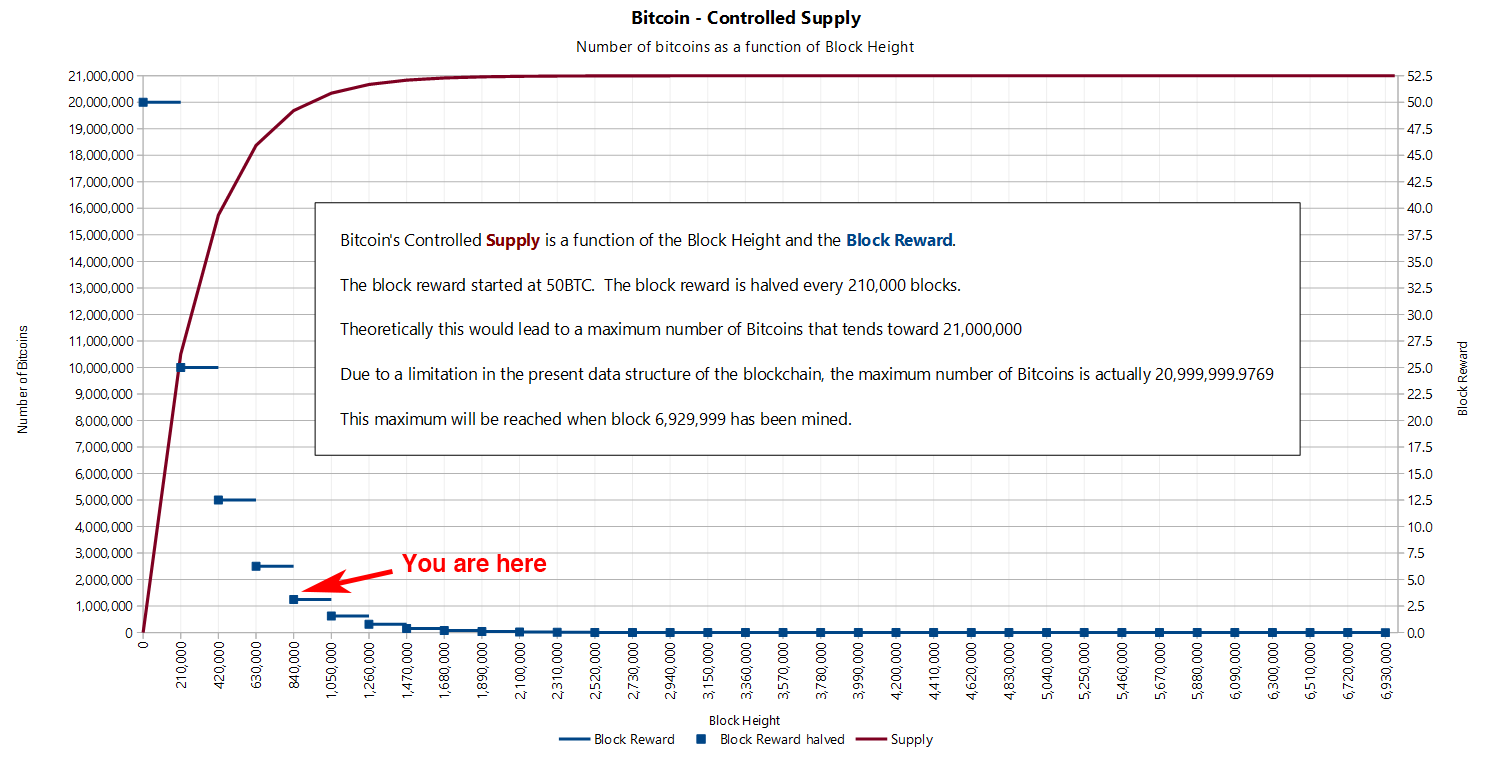
\includegraphics{assets/images/you-are-here.png}
  \caption{Suprimento controlado do Bitcoin}
  \label{fig:you-are-here.png}
\end{figure}

Fórmulas, funções logarítmicas e exponenciais não são intuitivas, e poucas pessoas conseguem entendê-las. O conceito da \textit{força} podeda moeda  ser mais fácil de entender se vista de outra forma. Uma vez que sabemos a quantidade de alguma coisa, e a dificuldade que é a sua produção ou como é difícil colocar as nossas mãos nisso, compreendemos imediatamente seu valor. O que é verdade para as pinturas do Picasso, para os violões de Elvis Presley e para os violinos Stradivarius também é verdade para a moeda fiduciária, ouro e bitcoins.

A dureza da moeda fiduciária depende de quem é o responsável pelas respectivas impressoras. Alguns governos podem estar mais dispostos a imprimir grandes quantidades de moeda do que outros, resultando em uma moeda mais fraca. Outros governos podem ser mais restritivos na impressão de dinheiro, resultando em moeda mais forte.

\begin{samepage}\begin{quotation}
\enquote{Um aspecto importante desta nova realidade é que instituições como o Fed não podem ir à falência. Eles podem imprimir qualquer quantia de dinheiro que eles podem precisar para si mesmos a um custo virtual próximo de zero.}
\begin{flushright} -- Jörg Guido Hülsmann\footnote{Jörg Guido Hülsmann, \textit{A Ética da Produção da Moeda}~\cite{hulsmann2008ethics}}
\end{flushright}\end{quotation}\end{samepage}

Antes de termos moedas fiduciárias, a solidez do dinheiro era determinada pelas propriedades naturais do material que usávamos como moeda. A quantidade de ouro na terra é limitada pelas leis da física. O ouro é raro porque supernovas e colisões de estrelas de nêutrons são raras. O \enquote{fluxo} de ouro é limitado porque extraí-lo da terra demanda um grande esforço. Por ser um elemento pesado, está principalmente enterrado no subsolo.

A abolição do padrão ouro deu lugar a uma nova realidade: adicionar dinheiro novo requer apenas uma gota de tinta. Em nosso mundo moderno, adicionar alguns zeros ao saldo de uma conta bancária exige ainda menos esforço: adicionar alguns bits em um computador de um banco é o suficiente.

O princípio delineado acima pode ser expresso de forma mais geral como a proporção de \enquote{estoque} em relação ao \enquote{fluxo}. Simplificando, o \textit{estoque} é quanto de algo temos atualmente. Para nossos propósitos, o estoque é uma medida da oferta monetária atual. O \textit{fluxo} é o quanto é produzido durante um período de tempo (por exemplo, em um ano). A chave para entender o dinheiro forte é entender essa relação entre estoque/fluxo (também conhecida como stock-to-flow, ou pelo sua abreviação S2F).

Calcular a relação estoque/fluxo de uma moeda fiduciária é difícil, porque quanto dinheiro existe depende de como você olhamos para ele.~\cite{wiki:money-supply} Você poderia contar apenas as notas e moedas (M0), adicione cheques e depósitos bancários (M1), adicionar contas de poupança e fundos mútuos e algumas outras coisas mais (M2), e ainda adicionar certificados de depósito a tudo isso (M3). Além disso, como tudo isso é definido e medido varia de país para país e como o Federal Reserve dos EUA parou de publicar os números \cite{web:fed-m3} para o M3, teremos que nos contentar com o suprimento monetário de M2. Eu adoraria verificar esses números, mas acho que temos que confiar no Fed por enquanto.

O ouro, um dos metais mais raros da Terra, tem a maior relação estoque/fluxo. De acordo com o US Geological Survey, um pouco mais de 190.000 toneladas foram extraídas. Nos últimos anos, cerca de 3.100 toneladas de ouro foram extraídas por ano.~\cite{mineral-commodity-summaries}

Usando esses números, podemos calcular facilmente a razão estoque/fluxo do ouro (ver Figura ~\ref{fig:stock-to-flow-gold}).

\begin{figure}
  \centering
  \begin{equation}
  \frac{190,000 t}{3,100 t} = ~ 61
  \end{equation}
  \caption{Razão do Stock-to-flow do Ouro}
  \label{fig:stock-to-flow-gold}
\end{figure}

Nada tem uma relação estoque/fluxo mais alta do que o ouro. É por isso que o ouro, até agora, era o dinheiro mais forte e sólido que existia. Costuma-se dizer que todo o ouro extraído até agora caberia em duas piscinas olímpicas. De acordo com meus cálculos\footnote{\url{https://bit.ly/gold-pools}}, precisaríamos de quatro. Talvez seja necessário atualizar essas informações ou as piscinas olímpicas ficaram menores.

Falando sobre o Bitcoin. Como você provavelmente sabe, a mineração de bitcoin esteve na moda nos últimos dois anos. Isso ocorre porque ainda estamos nas fases iniciais do que é chamado de \textit{era da recompensa}, onde os nodes de mineração são recompensados com \textit{muito} bitcoin por seu esforço computacional. Atualmente, estamos na era de recompensa número 4, que começou em 2020 e terminará no início de 2024, provavelmente em maio. Embora o suprimento de bitcoin seja predeterminado, o funcionamento interno do Bitcoin permite apenas datas aproximadas. No entanto, podemos prever com certeza quão alta será a relação estoque/fluxo do Bitcoin. Alerta de spoiler: Será alto.

Quão alto? Bem, acontece que o Bitcoin ficará infinitamente difícil (veja a Figura~\ref{fig:stock-to-flow-white-cropped}).

\begin{figure}
  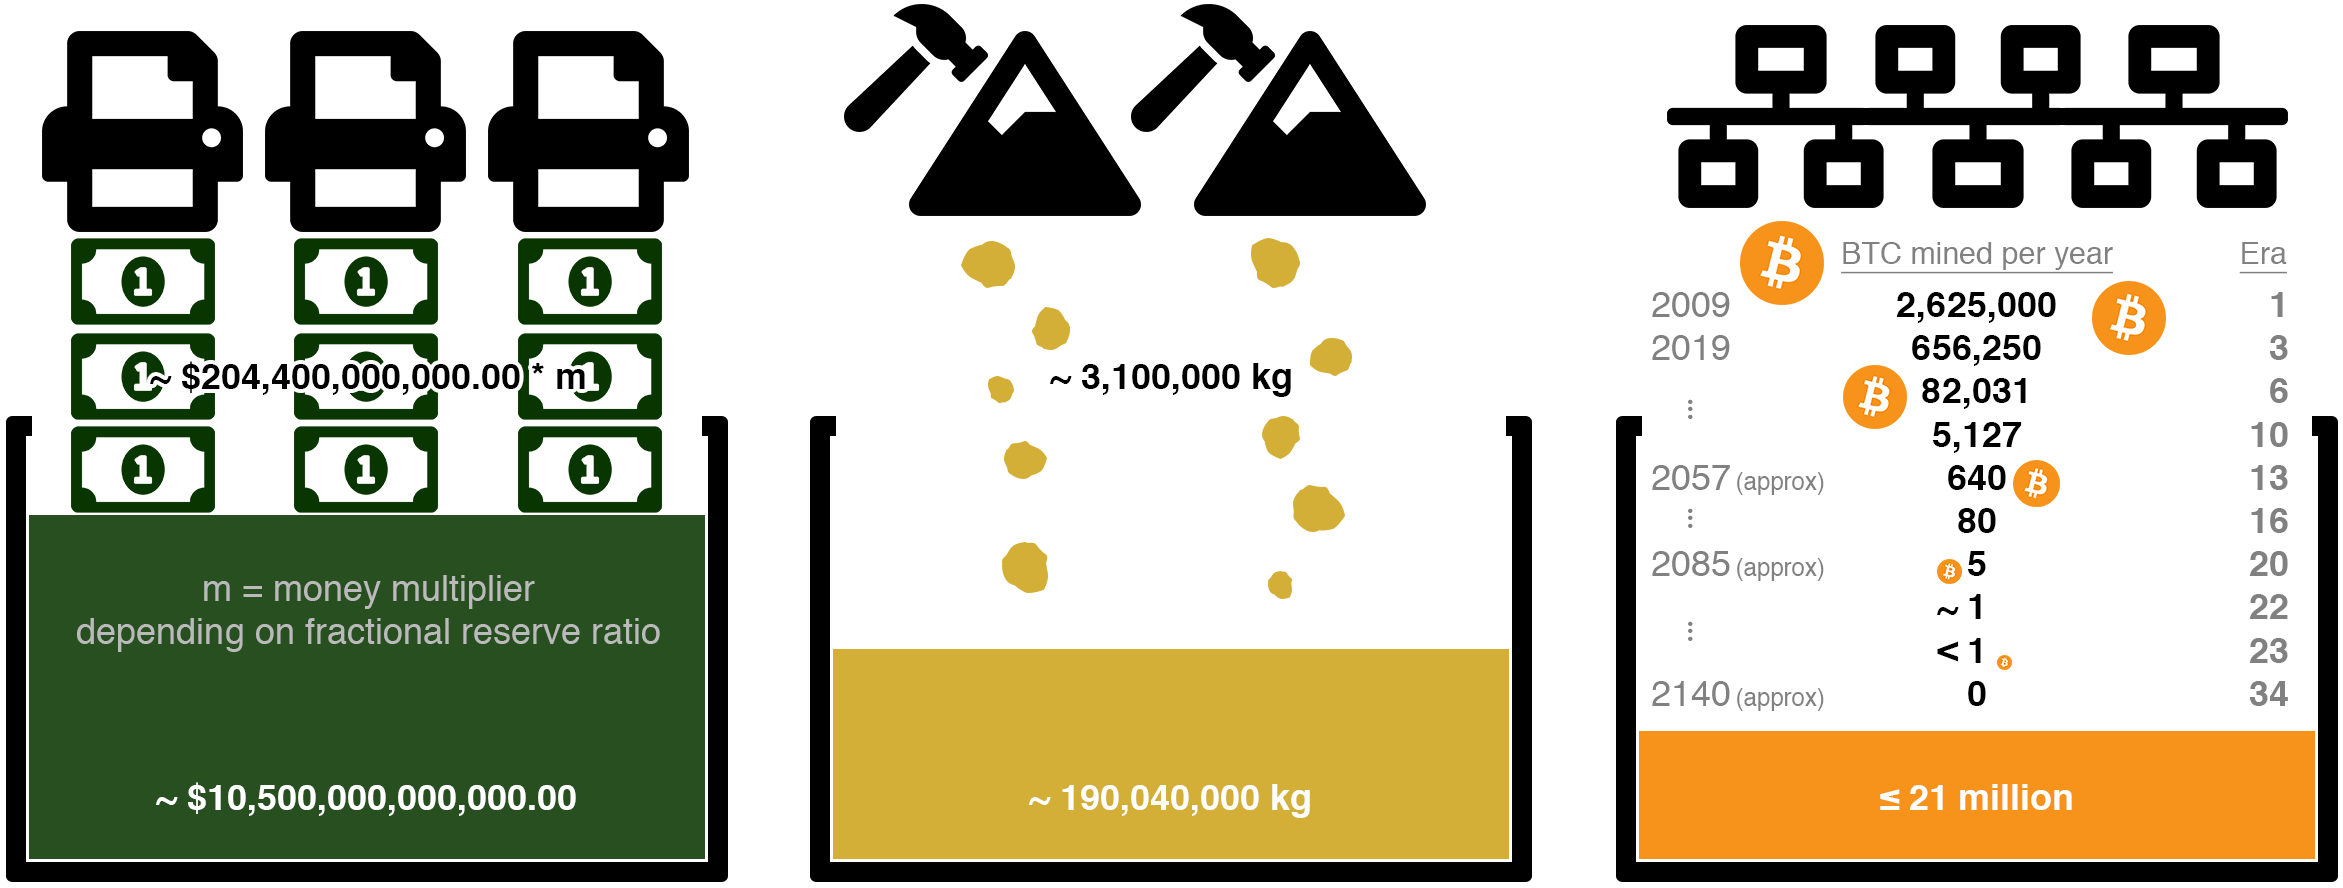
\includegraphics{assets/images/stock-to-flow-white-cropped.png}
  \caption{Visualização de estoque e do fluxo de USD, ouro e Bitcoin}
  \label{fig:stock-to-flow-white-cropped}
\end{figure}

\paragraph{}
Devido a uma diminuição exponencial da recompensa de mineração, o fluxo de novo bitcoin diminuirá, resultando em uma relação estoque/fluxo vertiginosa. Ele alcançará o ouro em 2020, apenas para superá-lo quatro anos depois, dobrando sua força novamente. Essa duplicação ocorrerá 64 vezes no total. Graças ao poder dos exponenciais, o número de bitcoin extraído por ano cairá abaixo de 100 bitcoin em 50 anos e abaixo de 1 bitcoin em 75 anos. A torneira global que é a recompensa em bloco vai secar por volta do ano 2140, parando efetivamente a produção de novos bitcoins. Este é um longo jogo. Se você está lendo isso, você ainda está no começo.

\begin{figure}
  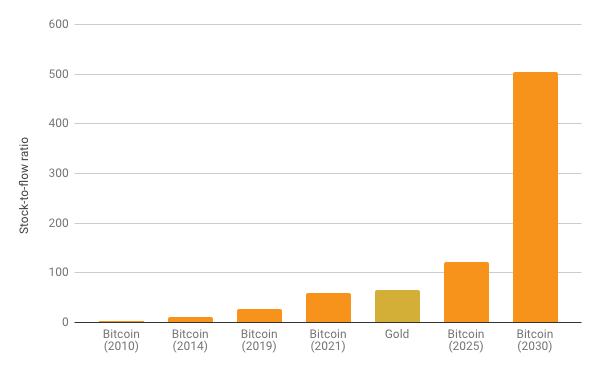
\includegraphics{assets/images/soundness-over-time.png}
  \caption{Aumento da razão estoque-fluxo do bitcoin em comparação com o ouro}
  \label{fig:soundness-over-time}
\end{figure}

À medida que o bitcoin se aproxima da proporção infinita de estoque e fluxo, será o dinheiro mais forte que existe. A solidez infinita é difícil de vencer.

Visto pelas lentes da economia, o \textit{ajuste de dificuldade} do Bitcoin é provavelmente seu componente mais importante. O quão difícil é extrair bitcoins depende da rapidez com que novos bitcoins são extraídos. \footnote{Na verdade, depende da rapidez com que blocos válidos são encontrados, mas para nossos propósitos, isso é a mesma coisa que \enquote{minerar bitcoins} e será assim, pelos próximos 120 anos.} É o ajuste dinâmico da dificuldade de mineração da rede que nos permite prever seu suprimento futuro.

A simplicidade do algoritmo de ajuste de dificuldade pode desviar a atenção de sua profundidade, mas o ajuste de dificuldade é realmente uma revolução de proporções einsteinianas. Isso garante que, não importa quanto ou quão pouco esforço seja gasto na mineração, o fornecimento controlado de Bitcoin não será interrompido. Ao contrário de todos os outros recursos, não importa quanta energia alguém coloque na mineração de bitcoins, a recompensa total não aumentará.

Assim como $E=mc^2$ dita o limite de velocidade universal em nosso universo, o ajuste de dificuldade do Bitcoin dita o \textbf{limite de dinheiro universal} no Bitcoin.

\paragraph{}
Se não fosse por esse ajuste de dificuldade, todos os bitcoins já teriam sido minerados. Se não fosse por esse ajuste de dificuldade, o Bitcoin provavelmente não teria sobrevivido a sua infância. É o que protege a rede em sua era de recompensa. É o que garante uma distribuição estável e justa\footnote{Dan Held, \textit{A distribuição do Bitcoin era justa}~\cite{distribution-was-fair}} do novo bitcoin. É o termostato que regula a política monetária do Bitcoin.

Einstein nos mostrou algo novo: não importa o quanto você empurre um objeto, em certo ponto você não conseguirá obter mais velocidade com ele. Satoshi também nos mostrou algo novo: não importa o quanto você procure por esse ouro digital, em certo ponto você não conseguirá extrair mais bitcoins dele. Pela primeira vez na história da humanidade, temos um bem monetário do qual, não importa o quanto você tente, você não será capaz de produzir mais.

\paragraph{O Bitcoin me ensinou que dinheiro forte é essencial.}

% ---
%
% #### Through the Looking-Glass
%
% - [Bitcoin's Energy Consumption: A Shift in Perspective][much energy]
%
% #### Down the Rabbit Hole
%
% - [The Ethics of Money Production][Jörg Guido Hülsmann] by Jörg Guido Hülsmann
% - [Mineral Commodity Summaries 2019][last few years] by the United States Geological Survey
% - [Bitcoin’s Distribution was Fair][fair distribution] by Dan Held
% - [Bitcoin's Controlled Supply][algorithmically controlled] on the Bitcoin Wiki
% - [Money Supply][how much money there is], [Speed of Light][universal speed limit] on Wikipedia
%
% <!-- Internal -->
% [much energy]: 
%
% [Fr. Bernard W. Dempsey, S.J.]: https://www.jstor.org/stable/29769582
% [Jörg Guido Hülsmann]: https://mises.org/sites/default/files/The%20Ethics%20of%20Money%20Production_2.pdf
% [stopped publishing]: https://www.federalreserve.gov/Releases/h6/discm3.htm
% [last few years]: https://minerals.usgs.gov/minerals/pubs/mcs/2018/mcs2018.pdf
% [my calculations]: https://www.wolframalpha.com/input/?i=volume+of+190000+metric+tons+gold+%2F+olympic+swimming+pool+volume
% [fair distribution]: https://blog.picks.co/bitcoins-distribution-was-fair-e2ef7bbbc892
%
% <!-- Bitcoin Wiki -->
% [algorithmically controlled]: https://en.bitcoin.it/wiki/Controlled_supply
%
% <!-- Wikipedia -->
% [how much money there is]: https://en.wikipedia.org/wiki/Money_supply
% [universal speed limit]: https://en.wikipedia.org/wiki/Speed_of_light#Upper_limit_on_speeds
% [alice]: https://en.wikipedia.org/wiki/Alice%27s_Adventures_in_Wonderland
% [carroll]: https://en.wikipedia.org/wiki/Lewis_Carroll
